\documentclass{article}
\usepackage{amsmath}
\usepackage{amsthm}
\usepackage{amssymb}
\usepackage{algorithm}
\usepackage{graphicx}
\usepackage[noend]{algpseudocode}
\usepackage{url}

\newlength\tindent
\setlength{\tindent}{\parindent}
\setlength{\parindent}{0pt}
\renewcommand{\indent}{\hspace*{\tindent}}

\newtheorem{thm}{Theorem}
\newtheorem{cor}{Corollary}[thm]
\newtheorem{lemma}{Lemma}[thm]

\title{Job Scheduling Problem}
\author{Daniel Braithwaite}

\begin{document}
	\pagenumbering{gobble}
	\maketitle
	\newpage
  	\pagenumbering{arabic}
  			
	\section{Deterministic Algorithm}
		\subsection{Approximation Ratio}
			Say we have $m$ computers, we start by assuming our scheduler has been given $m$ simple jobs, assuming our algorithm wants to be optimal and considering that we cant see what is coming next we will assign one of these simple jobs to each of the $m$ machines. Now that it has scheduled the simple jobs we give it a single complex job. No matter which machine we assign the complex job to we end up with a total cost of 15 minutes where we could have a total cost of 10 minutes.\newline
			
			This gives us an approximation ratio of $\frac{15}{10} = 1.5$.
			
			\begin{lemma}
				No deterministic algorithm online algorithm for scheduling jobs can have a better ratio than 1.5
			\end{lemma}
			
			\begin{proof}
				We assume that our algorithm is always making the optimal choice when given a job. We clearly will want to assign incoming jobs to computers that don't already have a job on them. So we see we will assign the $m$ simple jobs to each of the $m$ computers. Given that we don't know about incoming jobs we cant arrange the tasks differently if the last one to be received is a complex job. So this leaves us with a solution with a cost of 15. Giving us a ratio of 1.5
			\end{proof}
				
		\subsection{Algorithm}
			We want to design an algorithm with the best approximation ratio of 1.5. We can see how we want to do this by referencing the proof in the previous section. We just want to assign the incoming job to the machine with the least total time as this will give us the best distribution across the machines.\newline
		
			We only have one input for the algorithm which is the machines. Assume we have a method that gives us the next job $getNextJob()$, and a method that tells us if we have any jobs left $haveJobsLeft()$	
		
			\begin{algorithm}
				\begin{algorithmic}[1]
					\Procedure{deterministicJobSchedule}{$m$}
						\While{$haveJobsLeft()$}
							\State $j \gets getNextJob()$
							\State $i \gets$ machine with smallest queue
							\State assign j to $m[i]$
						\EndWhile
					\EndProcedure
				\end{algorithmic}
			\end{algorithm}
	
		\subsection{Complexity}
			Say we have $n$ jobs, then the outer loop will repeat $n$ times. Along with this we see that finding the machine with the smallest queue requires us to iterate through all the machines which will take $m$ steps where $m$ is the number of machines we have. Giving us a total complexity of
			
			\begin{align*}
				\theta(nm)
			\end{align*}
					
		\subsection{Testing}
			When testing this algorithm I generated worst case input to graph so that we could see the algorithm had an approximation ratio of 1.5. I also tested the program on randomly generated data with three different numbers of machines (5, 10, 20) so we could see that the algorithm never exceeded the approximation ratio of 1.5. As we can see in the graph below both these things hold and that the approximation ratio is as expected.
			
			\begin{figure}[h]
				\vspace{3mm}
				\begin{center}
					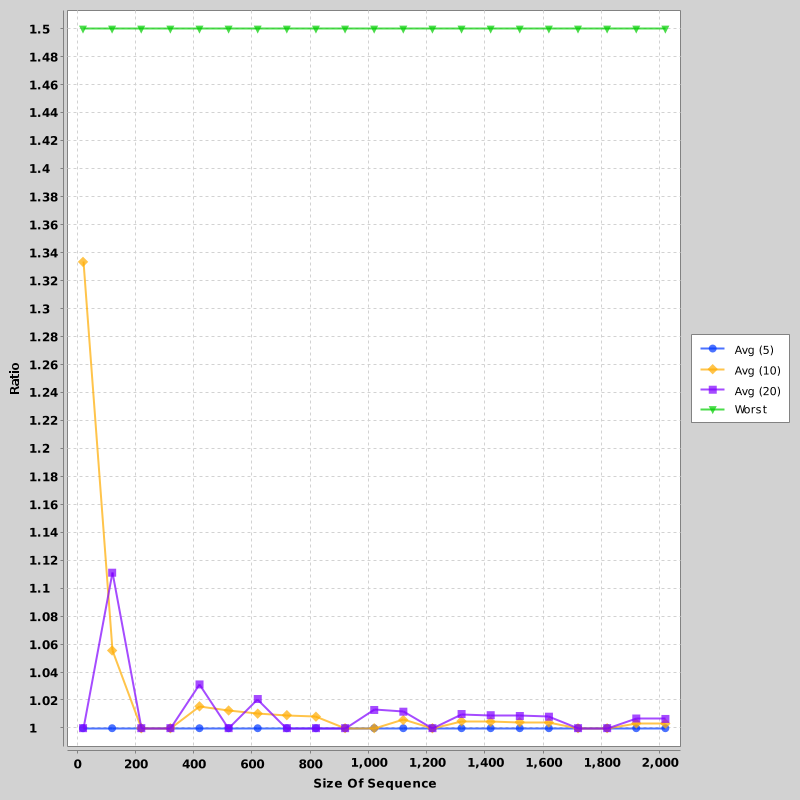
\includegraphics[scale=0.4]{Approx.png}
				\end{center}
			\end{figure}
		
		
	\section{Probabilistic Algorithm}				
		\subsection{Algorithm}
			For this algorithm I am randomly assigning simple tasks and deterministic assigning complex tasks. This was because since complex tasks are bigger randomly assigning them will have more chance of making an issue where as simple tasks in the wrong place wont put out the solution by much. Assuming we are given a random distribution of simple and complex job this will also give us a significant speed increase from the deterministic algorithm\newline
		
			We will assume we have a method that gives us the next job $getNextJob()$, and a method that tells us if we have any jobs left $haveJobsLeft()$. Along with $uniformRandomInt(m)$, which returns a random number between 0 and m (not including m)
			\begin{algorithm}
				\begin{algorithmic}[1]
					\Procedure{probilisticJobSchedule}{$m$}
						\While{$haveJobsLeft()$}
							\State $j \gets getNextJob()$
							
							\If{$j$ is simple}
								\State $i \gets uniformRandomInt(m)$
							\Else
								\State $i \gets$ machine with smallest queue
							\EndIf
							
							\State assign j to $m[i]$
						\EndWhile
					\EndProcedure
				\end{algorithmic}
			\end{algorithm}	
	
		\subsection{Approximation Ratio}
			We see that the approximation ratio for our probabilistic algorithm is the same as that for the deterministic algorithm by the following reasoning using the same worst case scenario as before.\newline
			
			If we get given $m$ simple jobs then given that we are uniformly distributing them across the machines when we get given the complex job the only thing to do is put it on a computer with a simple job and get a total cost of 15. We know that the optimal solution is 10. Giving us the approximation ratio of 1.5.
	
		\subsection{Complexity}
			The loop for this algorithm will repeat $n$ times where we have $n$ jobs. The probabilistic part of this algorithm will have a constant time complexity. And the deterministic part will have a complexity of $m$ where $m$ is the number of machines. 
			
			\begin{align*}
				\theta(nm)
			\end{align*}
			
		\subsection{Testing}
			I tested this algorithm on random input and for each used three different numbers of machines. The solutions start of being wildly incorrect but as the input size grows the algorithm gets more accurate. The graph also shows that almost always having 5 machines will gives you better results than having 10 or 20. We can observer in the graph below that the approximation ratio is as we expected. We see that practically all of the plotted data falls below 1.5 and the few about can be explained by the fact that the expected ratio was calculated using the expected output of the algorithm, the fact that the algorithm is randomized means that we will sometimes get an output that is way off expected. 
			
			\begin{figure}[h]
				\vspace{3mm}
				\begin{center}
					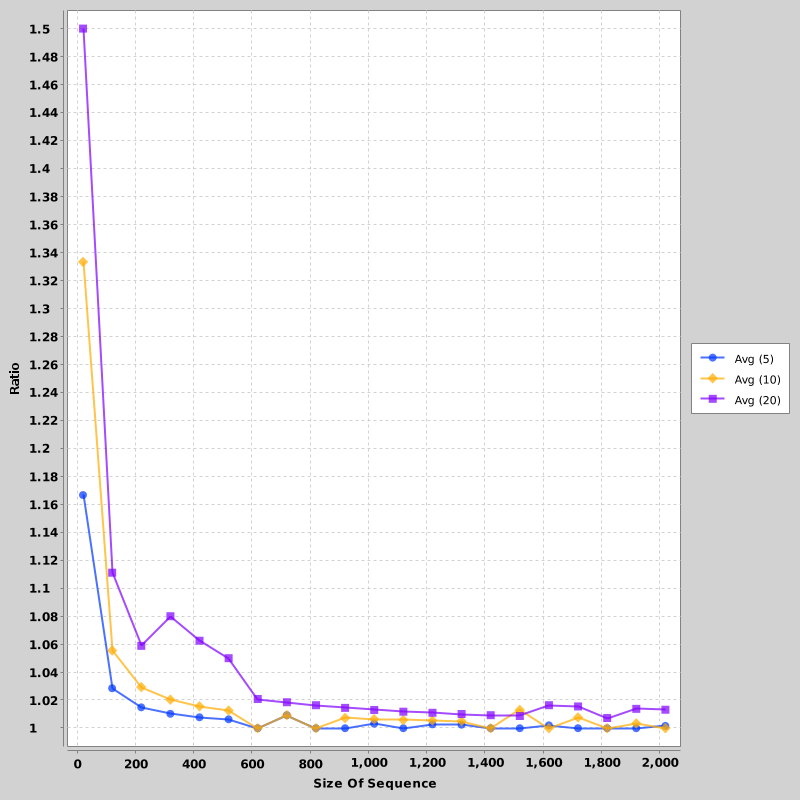
\includegraphics[scale=0.4]{Prob.png}
				\end{center}
			\end{figure}
			
			\break
			
	\section{Comparison}
		\subsection{Approximation Ratios}
			We can graph the approximation ratios of the two algorithms to see that deterministic algorithm out performs the probabilistic but not by a lot.
			
			\begin{figure}[h]
				\vspace{3mm}
				\begin{center}
					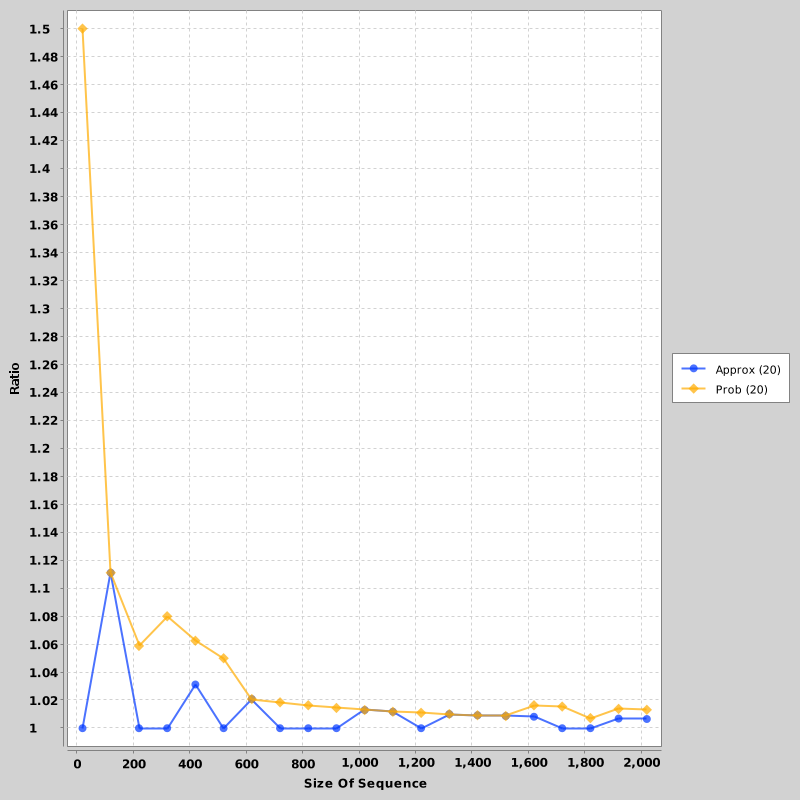
\includegraphics[scale=0.4]{CompareRatios.png}
				\end{center}
			\end{figure}
			
			\break
			
		\subsection{Complexity}
			If we compare the order cost of both the algorithms we see that the probabilistic algorithm and deterministic algorithms have the same order cost but if we examine the graph below we see that the probabilistic algorithmic out performs the deterministic one.
			
			\begin{figure}[h]
				\vspace{3mm}
				\begin{center}
					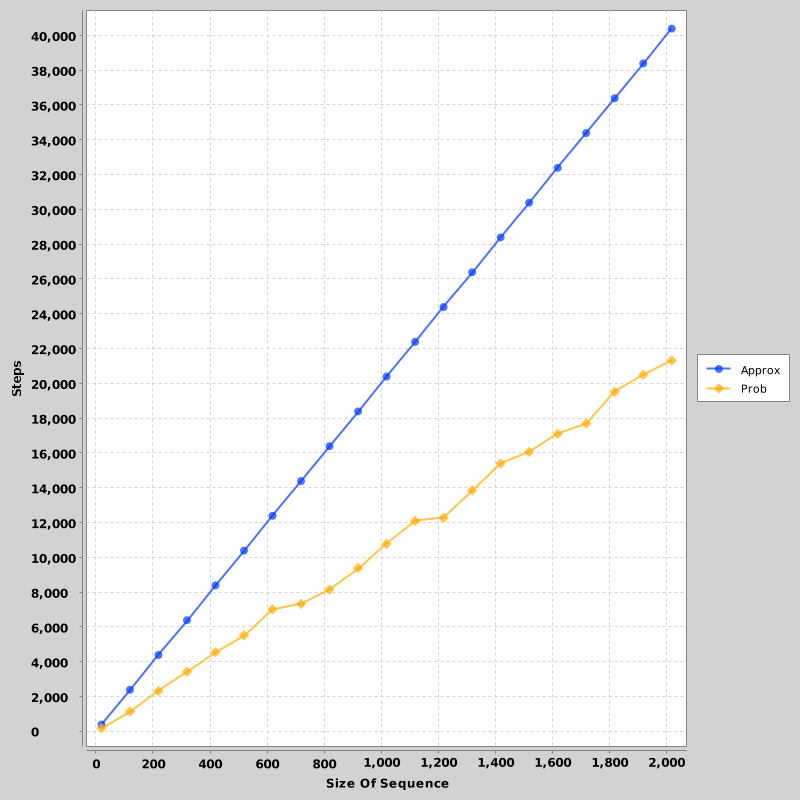
\includegraphics[scale=0.4]{CompareComplexity.png}
				\end{center}
			\end{figure}
			
			\break		
			
		\subsection{Summary}
			While the deterministic algorithm gives a consistently good solution most of the time it is only slightly better if not the same as the probabilistic algorithm. Along with this we see that the probabilistic algorithm is considerably faster than the deterministic one.\newline
			
			The key difference between the two is that the probabilistic one will randomly assign the simple tasks to machines, this hopefully causes enough variance in the solution so that we can avoid arriving at a sub optimal solution. By only randomly assigning the simple tasks we are introducing variation but also minimizing risk. If a simple task is randomly assigned to a bad position then the offset caused by that isn't as much as if we assigned a complex task to a bad position.
			
	\section{Alternative Solutions Considered}
		\subsection{Probabilistic Algorithm}
			One possible solution I considered was rather than only randomly assigning simple tasks, just randomly assign any task but only $\alpha$ percent of the time. However in testing this didn't perform as optimally as the solution given in this report.
			
	\section{Further Improvements}
		\subsection{Deterministic Algorithm}
			A simple way to improve the effective of the deterministic algorithm would be to use a heap to store the computers. This would give is $log(m)$ time instead of $m$ time (where $m$ is the number of machines)
		
  	
\end{document}